% -*- root: Dissertation.tex -*-
\documentclass[Dissertation.tex]{subfiles}
\graphicspath{{../Figures/}}
\begin{document}
\chapter{Entropy Norms for Compressible Navier-Stokes}
\label{sec:EntropyNorm}
\section{Motivation}

From the previous appendix, let $W$, $U$, and $V$ denote the set of primitive, conservation, and
entropy variables respectively.
% Define entropy function
It is well known that the entropy function
\[
H=-\rho\log(p\rho^{-\gamma})\,.
\]
provides a natural residual for the system of equations.
The Hessian of $H$ is known as the symmetrizer of the Navier-Stokes system
$A_0=H_{,UU}$, and $(U,A_0U)$ provides a physically consistent, entropy based metric.
By definition of the entropy variables (see \cite{HughesEntropyVariables}) $V_{,U}=H_{,UU}$, where
\[
V_{,U}(U)=\arrthree
{\frac{4\gamma\rho^2E^2-4\gamma\rho E\bfm\cdot\bfm+(1+\gamma)(\bfm\cdot\bfm)^2}{\rho(\bfm\cdot\bfm-2\rho E)^2}}
{-\frac{2\bfm\bfm\cdot\bfm}{\LRp{\bfm\cdot\bfm-2\rho E}^2}}
{-\frac{4\rho(\rho E-\bfm\cdot\bfm)}{\LRp{\bfm\cdot\bfm-2\rho E}^2}}
{}
{\frac{2\rho(2\rho E+\bfm\cdot\bfm)}{\LRp{\bfm\cdot\bfm-2\rho E}^2}}
{-\frac{4\rho^2\bfm}{\LRp{\bfm\cdot\bfm-2\rho E}^2}}
{Symm.}
{}
{\frac{4\rho^3}{\LRp{\bfm\cdot\bfm-2\rho E}^2}}\,.
\]

Since our previous comparison of Navier-Stokes formulations showed no strong reason to 
prefer anything over primitive variables, we will choose to work with primitive variables 
in this appendix. 
As such, we need to perform a change of variables to find the symmetrizer for the set of primitive variables:
% Consider a change of variables to primitive variables: 
$U=U_{,W}W$.
Our entropy metric is then
\[
\LRp{U_{,W} W,V_{,U}U_{,W} W}=\LRp{ W,U_{,W}^TV_{,U}U_{,W} W}
\]
Then
\[
U_{,W}=\arrthree{1}{0}{0}{\bfu}{\rho}{0}{C_vT+\frac{1}{2}\bfu\cdot\bfu}{\rho\bfu}{C_v\rho}
\]
where $V_{,U}$ in primitive variables is
\[
V_{,U}(W)=\arrthree
{\frac{\gamma}{\rho}+\frac{(\bfu\cdot\bfu)^2}{4\rho C_v^2 T^2}}
{-\frac{\frac{1}{2}\bfu\cdot\bfu\bfu}{\rho C_v^2 T^2}}
{-\frac{(C_v T-\frac{1}{2}\bfu\cdot\bfu)}{\rho C_v^2 T^2}}
{}
{\frac{C_v T+\bfu\cdot\bfu}{\rho C_v^2 T^2}}
{-\frac{\bfu}{\rho C_v^2 T^2}}
{Symm.}
{}
{\frac{1}{\rho C_v^2 T^2}}
\]
and
\[
A_0(W)=U_{,W}^TV_{,U}U_{,W}=\arrthree
{\frac{\gamma-1}{\rho}}
{0}
{0}
{0}
{\frac{\rho}{C_v T}}
{0}
{0}
{0}
{\frac{\rho}{T^2}}\,.
\]
As a check, $(W,A_0(W)W)$ has consistent units of density.
% Let $A_0^p=U_{,W}^TV_{,U}U_{,W}$ denote the symmetrizer for primitive variables.

\begin{figure}[ht]
\centering
\begin{subfigure}[t]{0.9\textwidth}
\centering
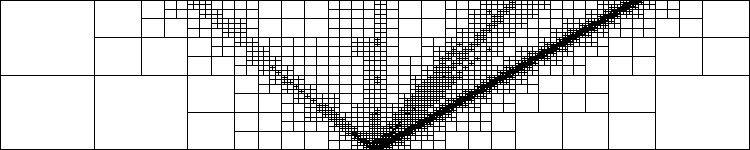
\includegraphics[width=\textwidth]{Dissertation/Sod/Robust-meshonly12.png}
\caption{Final mesh with robust norm}
\end{subfigure}
\begin{subfigure}[t]{0.9\textwidth}
\centering
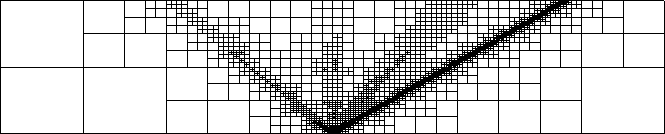
\includegraphics[width=\textwidth]{Dissertation/Sod/EntropyRobust-meshonly12.png}
\caption{Final mesh with entropy scaled robust norm}
\end{subfigure}
\begin{subfigure}[t]{0.9\textwidth}
\centering
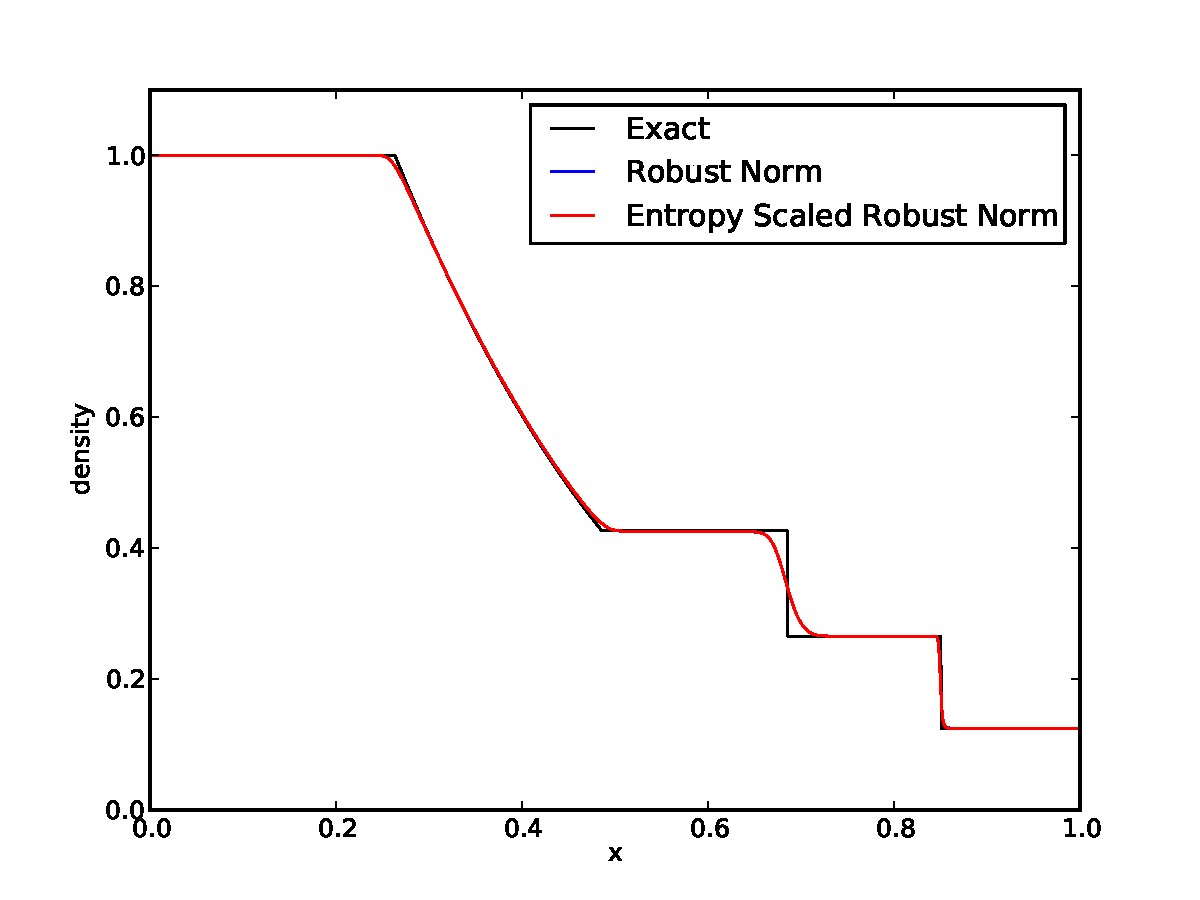
\includegraphics[width=\textwidth]{Dissertation/Sod/EntropyNormComparison-den.pdf}
\caption{Density at final time}
\end{subfigure}
\caption{Sod solution after 12 refinements}
\label{fig:SodEntropyComparison}
\end{figure}

\begin{figure}[ht]
\centering
\begin{subfigure}[t]{0.45\textwidth}
\centering

\includegraphics[width=\textwidth]{Dissertation/Noh/Robust-den10.png}
\caption{Final density with robust norm}
\end{subfigure}
\begin{subfigure}[t]{0.45\textwidth}
\centering
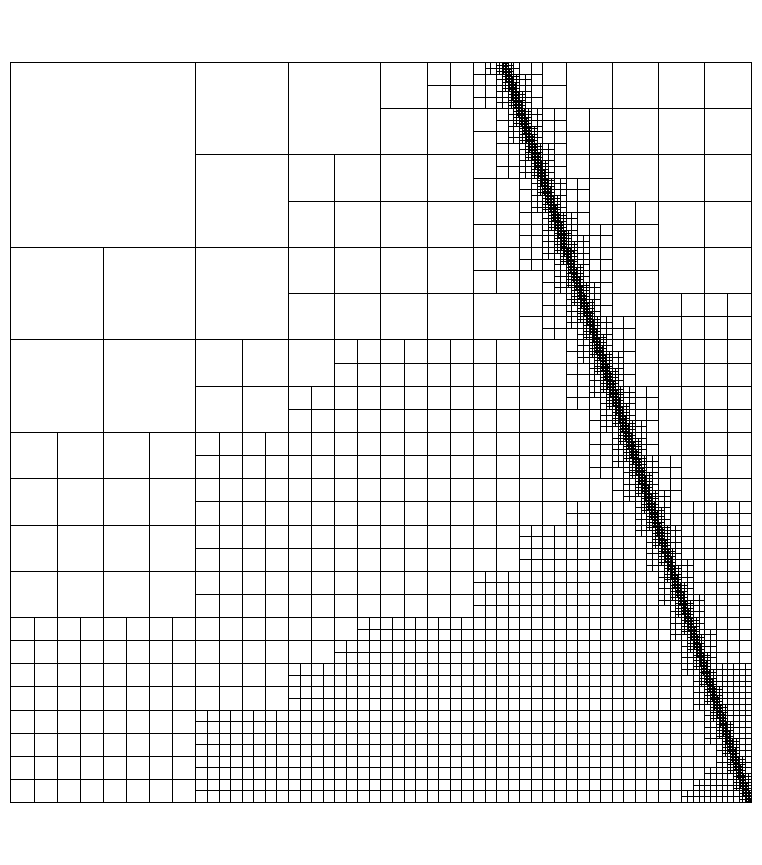
\includegraphics[width=\textwidth]{Dissertation/Noh/Robust-meshonly10.png}
\caption{Final mesh with robust norm}
\end{subfigure}
\begin{subfigure}[t]{0.45\textwidth}
\centering

\includegraphics[width=\textwidth]{Dissertation/Noh/EntropyRobust-den10.png}
\caption{Final density with entropy scaled robust norm}
\end{subfigure}
\begin{subfigure}[t]{0.45\textwidth}
\centering
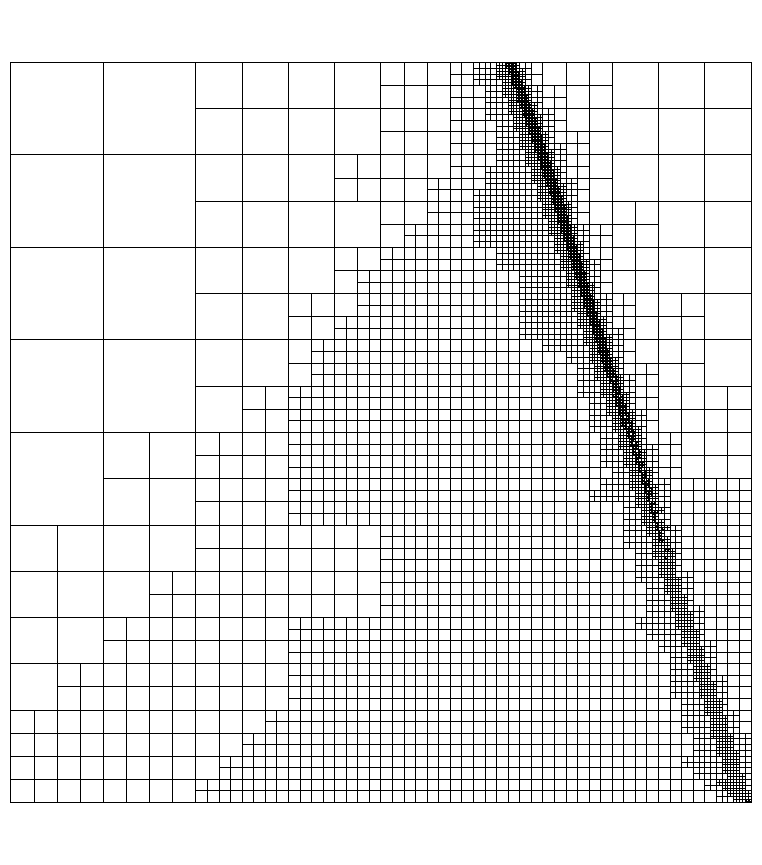
\includegraphics[width=\textwidth]{Dissertation/Noh/EntropyRobust-meshonly10.png}
\caption{Final mesh with entropy scaled robust norm}
\end{subfigure}
\caption{Noh solution after 10 refinements}
\label{fig:NohEntropyComparison}
\end{figure}

\begin{figure}[ht]
\centering
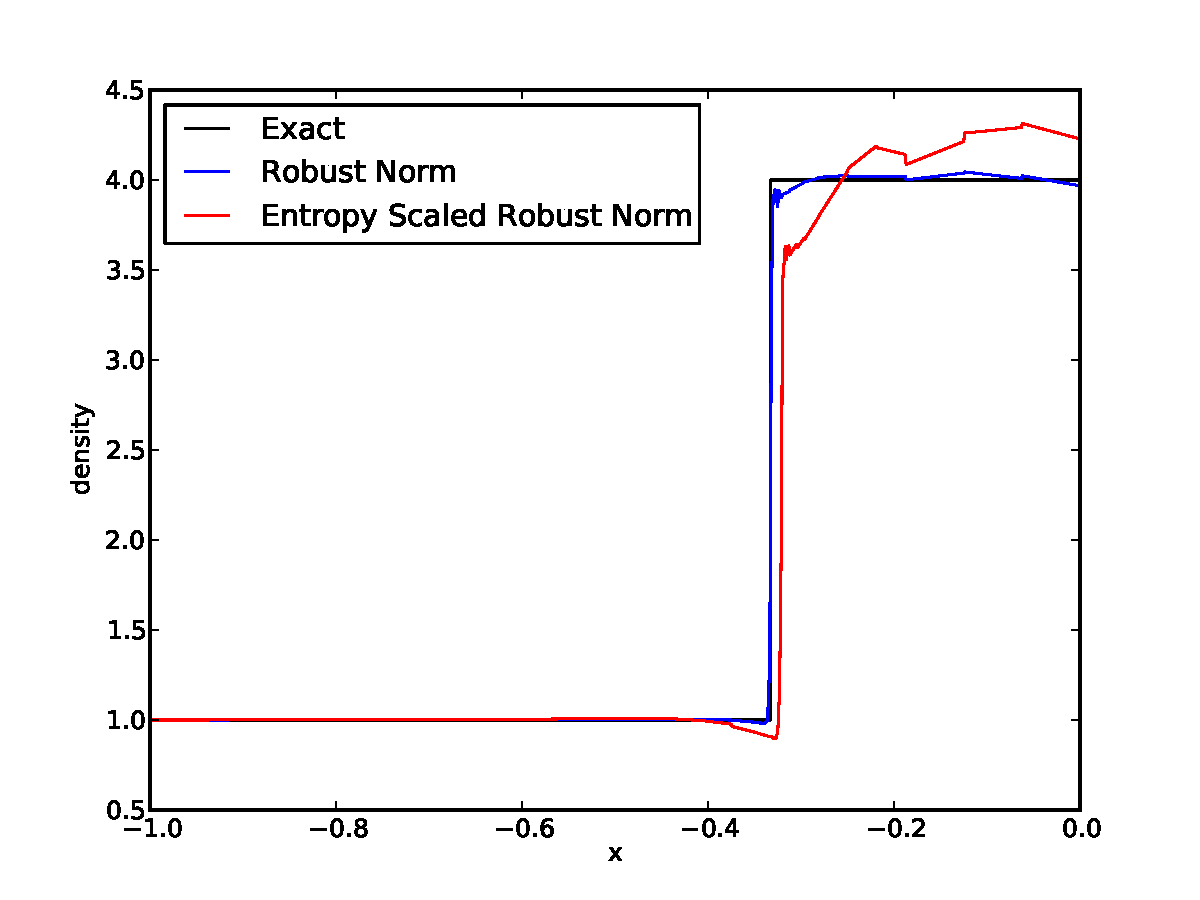
\includegraphics[width=0.9\textwidth]{Dissertation/Noh/EntropyNormComparison.pdf}
\caption{Density at final time}
\label{fig:NohEntropyComparison2}
\end{figure}

\end{document}
